\documentclass[12pt,a4paper]{article}

\usepackage[margin=2.5cm]{geometry}
\usepackage{graphicx}
\usepackage{caption}
\usepackage{subcaption}
\usepackage{hyperref}
\usepackage{booktabs}
\usepackage{parskip}
\usepackage{titlesec}
\usepackage{float}
\usepackage{xcolor}

\hypersetup{
    colorlinks=true,
    linkcolor=black,
    urlcolor=blue,
    citecolor=black
}

\titleformat{\section}{\large\bfseries}{}{0em}{}[\titlerule]
\titleformat{\subsection}{\normalsize\bfseries}{}{0em}{}

\title{
    \textbf{Cephalopod Behavioral Sentiment Analysis} \\
    \large GSoC 2026 Entry Task
}
\author{}
\date{}

\begin{document}

\maketitle

% ─────────────────────────────────────────────────────────────────────────────
\section{Introduction}

This report describes a simple video-based pipeline for inferring behavioral
state in cephalopods (specifically an octopus) from a short video clip.
The goal is to extract interpretable, frame-level features that serve as
proxies for locomotor activity and skin-pattern dynamics, visualise them over
time, and reason about what behavioral information they encode.

The video clip used is a 59-second segment (3:34–4:33) sourced from a
publicly available YouTube recording, downscaled to 1280$\times$720 px at
23.98 fps for efficient processing.

% ─────────────────────────────────────────────────────────────────────────────
\section{Behavioral Interpretation}

Motion magnitude tracks locomotor activity — separating rest from crawling, swimming, or escape jetting.
Histogram change captures chromatophore-driven skin patterning, which cephalopods use for camouflage and communication.
High values in both features together suggest active or defensive behaviour; high histogram change with low motion likely reflects stationary camouflage adjustment.
The main limitation is that both signals are computed over the full frame, so background movement and camera shake can mimic real animal activity.
Foreground segmentation or animal tracking would be needed to make the features truly animal-specific.
Adding a hydrophone would help detect jet propulsion bursts, and pose estimation would expose arm posture and mantle state — both strong indicators of behavioural intent.
A temporal model like an HMM or LSTM combining these signals could reliably segment behavioural states with much greater precision.

% ─────────────────────────────────────────────────────────────────────────────
\section{Features Extracted}

Two simple, interpretable features were chosen:

\begin{table}[H]
    \centering
    \begin{tabular}{lll}
        \toprule
        \textbf{\#} & \textbf{Feature} & \textbf{What it captures} \\
        \midrule
        1 & Frame-to-frame motion magnitude & Locomotor activity \\
        2 & Inter-frame histogram change & Chromatophore / skin-pattern dynamics \\
        \bottomrule
    \end{tabular}
    \caption{Extracted features and their behavioral interpretation.}
\end{table}

\subsection{Feature 1 — Motion Magnitude (Frame Differencing)}

For each consecutive pair of frames, both are converted to grayscale and the
mean absolute pixel difference is computed:

\[
    M_t = \frac{1}{WH} \sum_{x,y} \left| I_t(x,y) - I_{t-1}(x,y) \right|
\]

Higher values indicate more pixels changed between frames, i.e.\ more
physical movement in the scene.

\subsection{Feature 2 — Histogram Change}

A normalised 3-channel (BGR) histogram is computed for each frame. The
similarity between consecutive histograms is measured using Bhattacharyya
correlation, and the change score is defined as:

\[
    H_t = 1 - \text{corr}(\text{hist}_{t},\, \text{hist}_{t-1})
\]

A value of 0 means the frame is identical to the previous one; 1 means
maximal change. This feature is particularly relevant for cephalopods because
their chromatophores, iridophores, and papillae produce rapid, large-scale
colour and pattern shifts that are directly visible in the histogram.

Both signals are smoothed with a 0.4\,s uniform window to suppress
single-frame noise, then combined into a normalised \textbf{activity score}:

\[
    A_t = \frac{1}{2}\,\hat{M}_t + \frac{1}{2}\,\hat{H}_t
\]

where $\hat{\cdot}$ denotes min-max normalisation to $[0, 1]$.

% ─────────────────────────────────────────────────────────────────────────────
\section{Results}

\subsection{Behavioral Analysis Plot}

\begin{figure}[H]
    \centering
    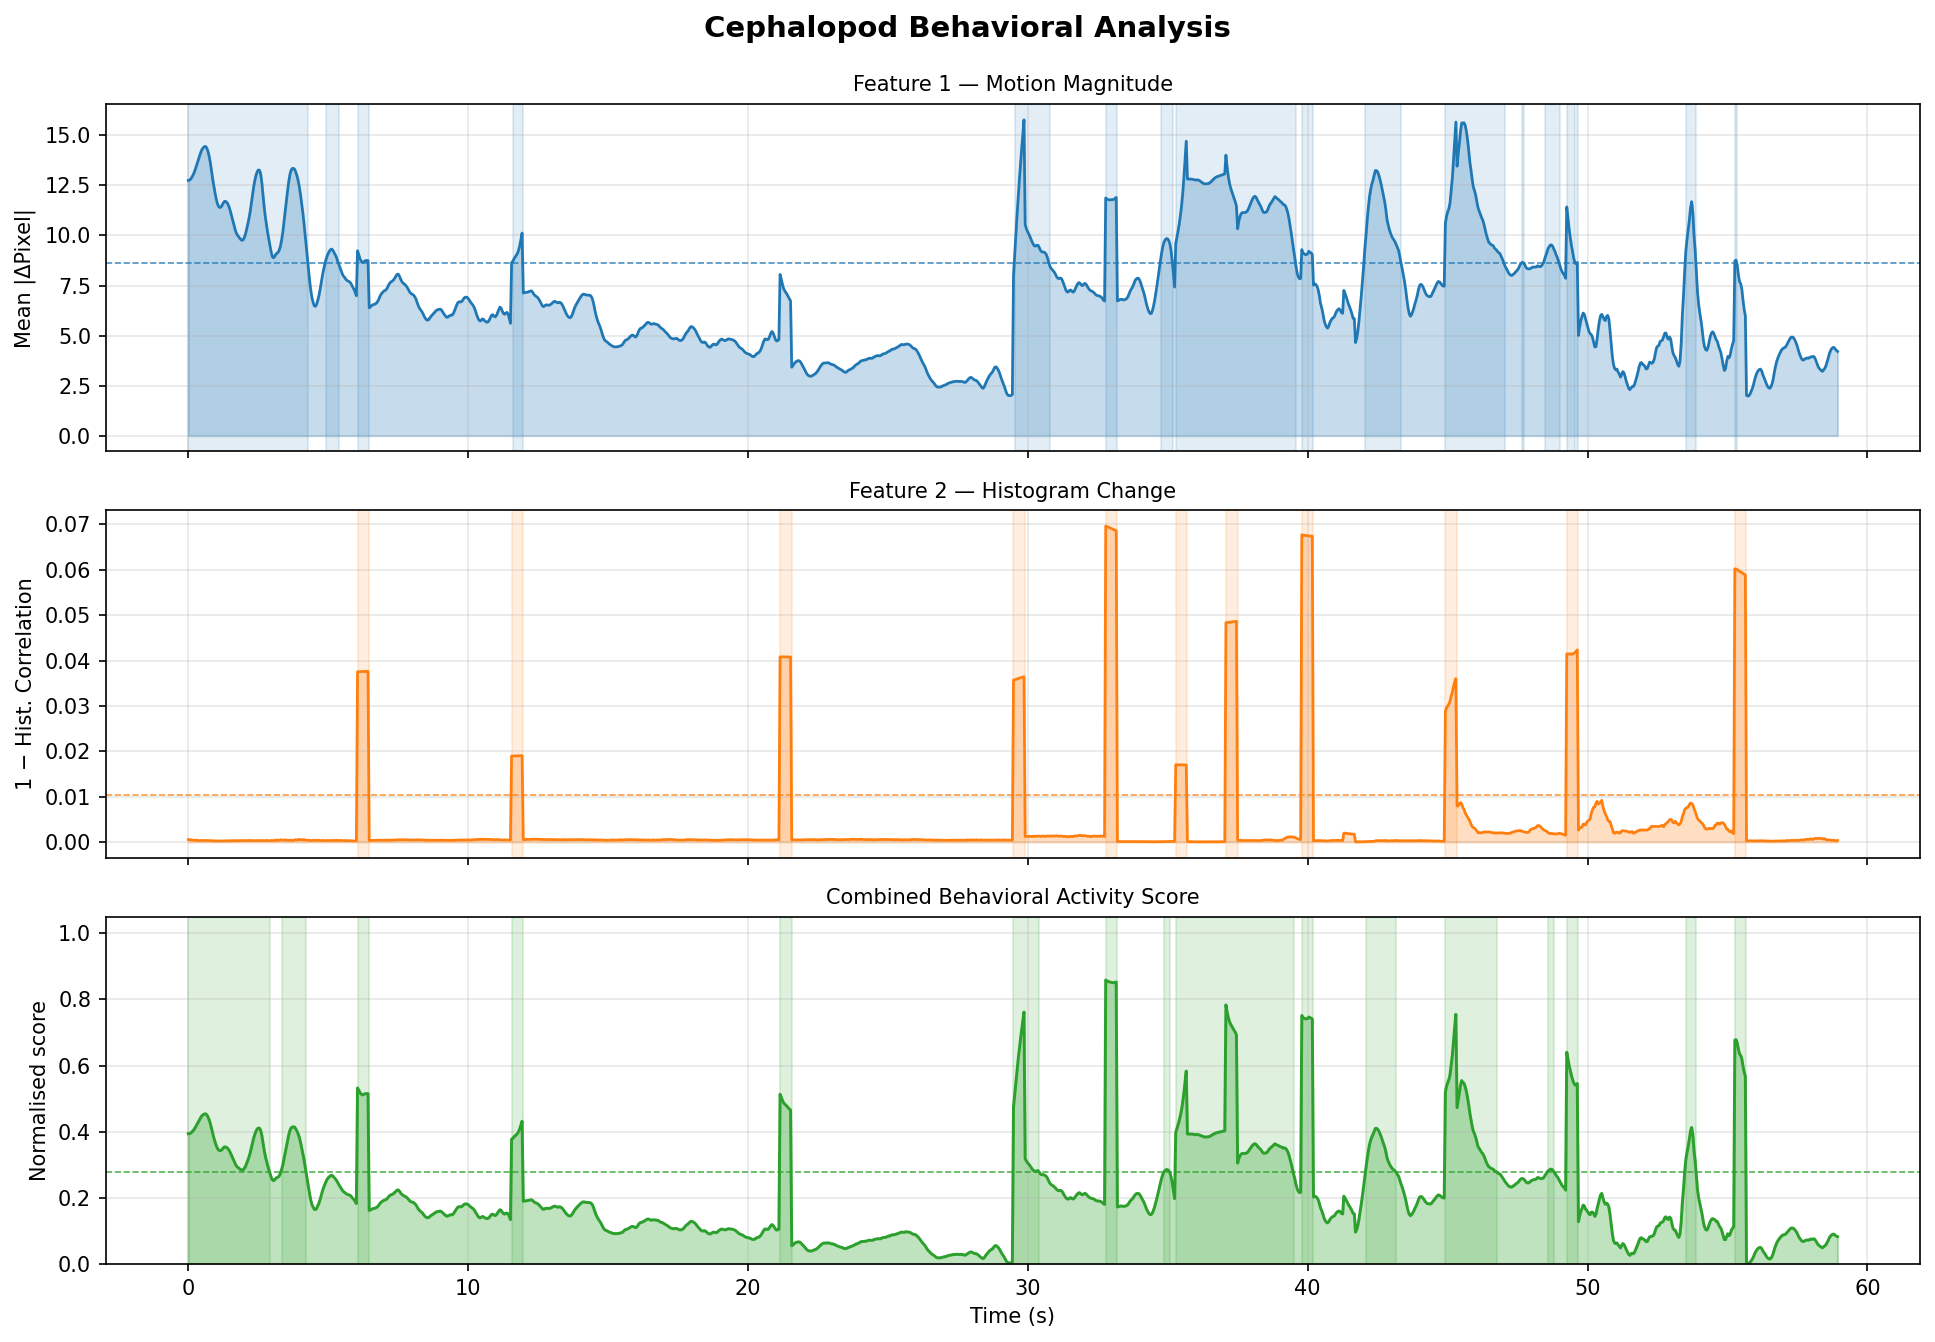
\includegraphics[width=\textwidth]{plots/data_octopus/behavioral_analysis.png}
    \caption{Three-panel behavioral analysis. Top: motion magnitude.
             Middle: histogram change. Bottom: combined activity score.
             Shaded spans mark periods exceeding the activity threshold
             (mean $+$ 0.4--0.5$\sigma$).}
\end{figure}

\subsection{Video Frame Preview}

\begin{figure}[H]
    \centering
    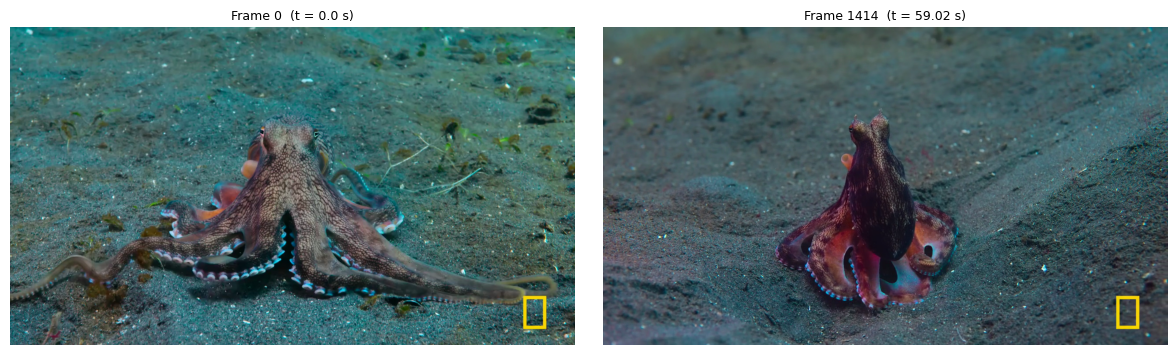
\includegraphics[width=\textwidth]{plots/data_octopus/frame_preview.png}
    \caption{First and last frame of the clip.}
\end{figure}

\subsection{High-Activity Frames}

\begin{figure}[H]
    \centering
    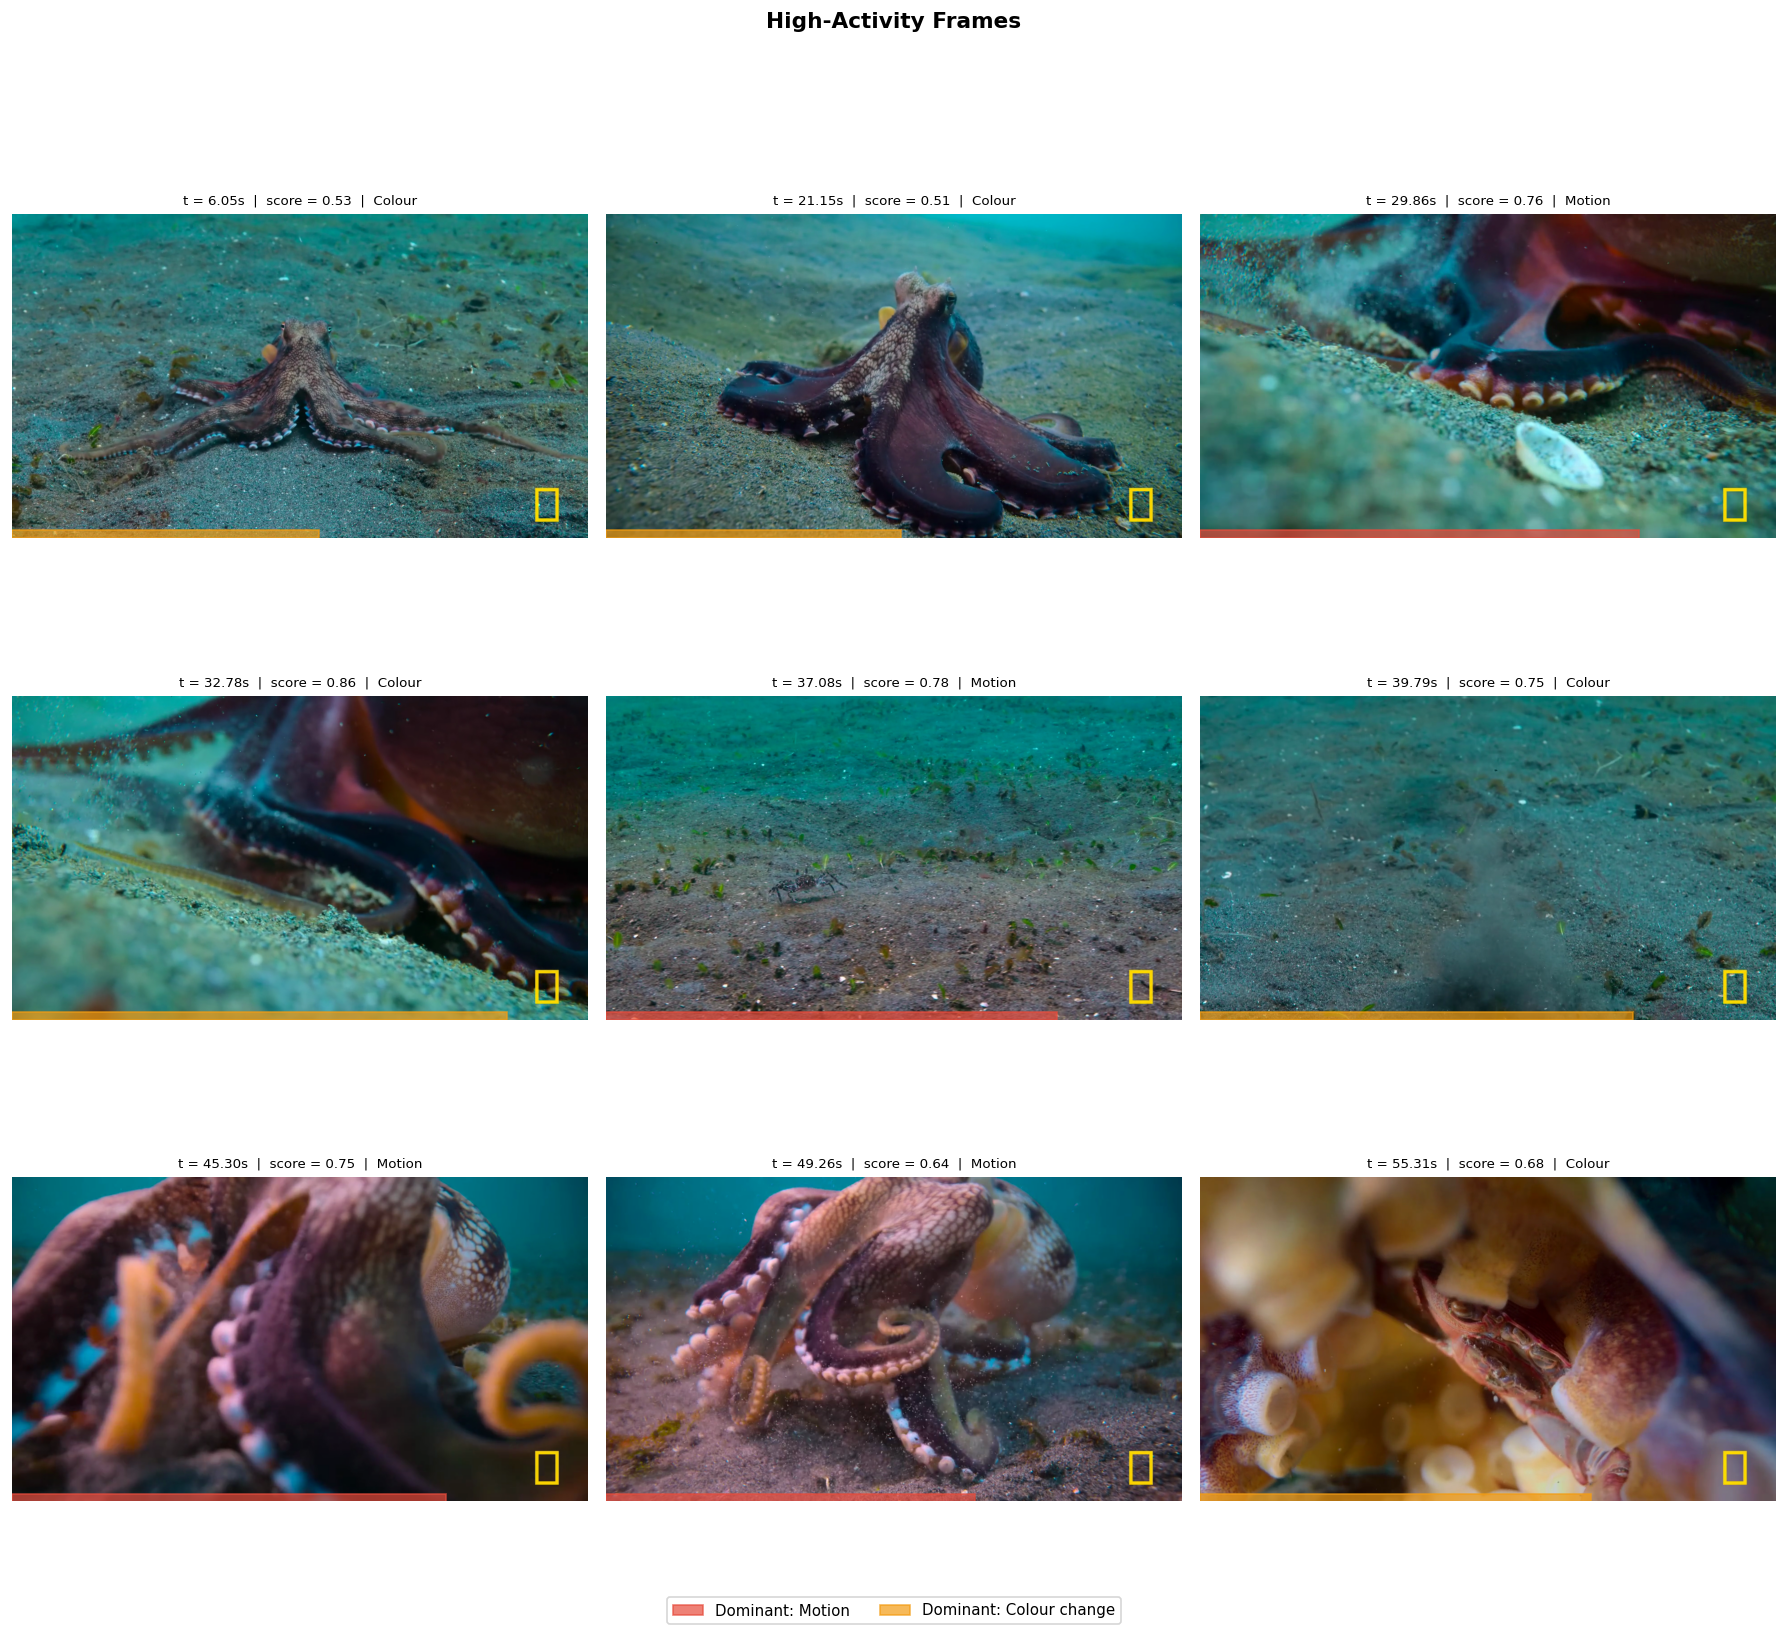
\includegraphics[width=\textwidth]{plots/data_octopus/activity_frames.png}
    \caption{Top 9 activity spikes with the actual video frame at each
             moment. Red bar indicates a motion-dominant event; orange
             indicates a colour-change-dominant event.}
\end{figure}

\subsection{Activity Event Table}

\begin{figure}[H]
    \centering
    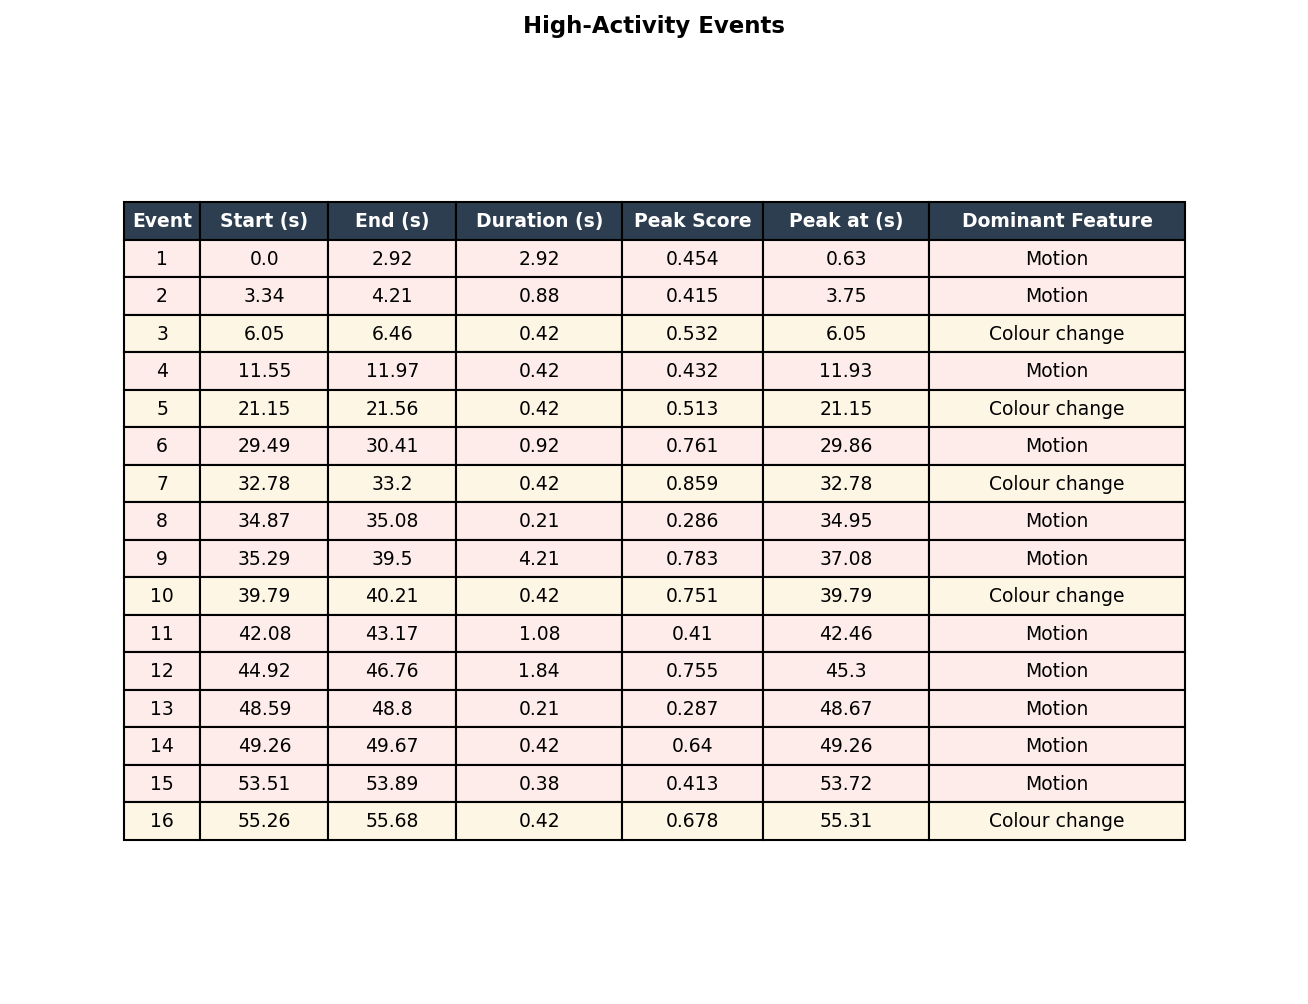
\includegraphics[width=\textwidth]{plots/data_octopus/activity_event_table.png}
    \caption{All contiguous high-activity events. Each row lists the start
             time, end time, duration, peak score, and dominant feature.}
\end{figure}

\subsection{Activity Timeline}

\begin{figure}[H]
    \centering
    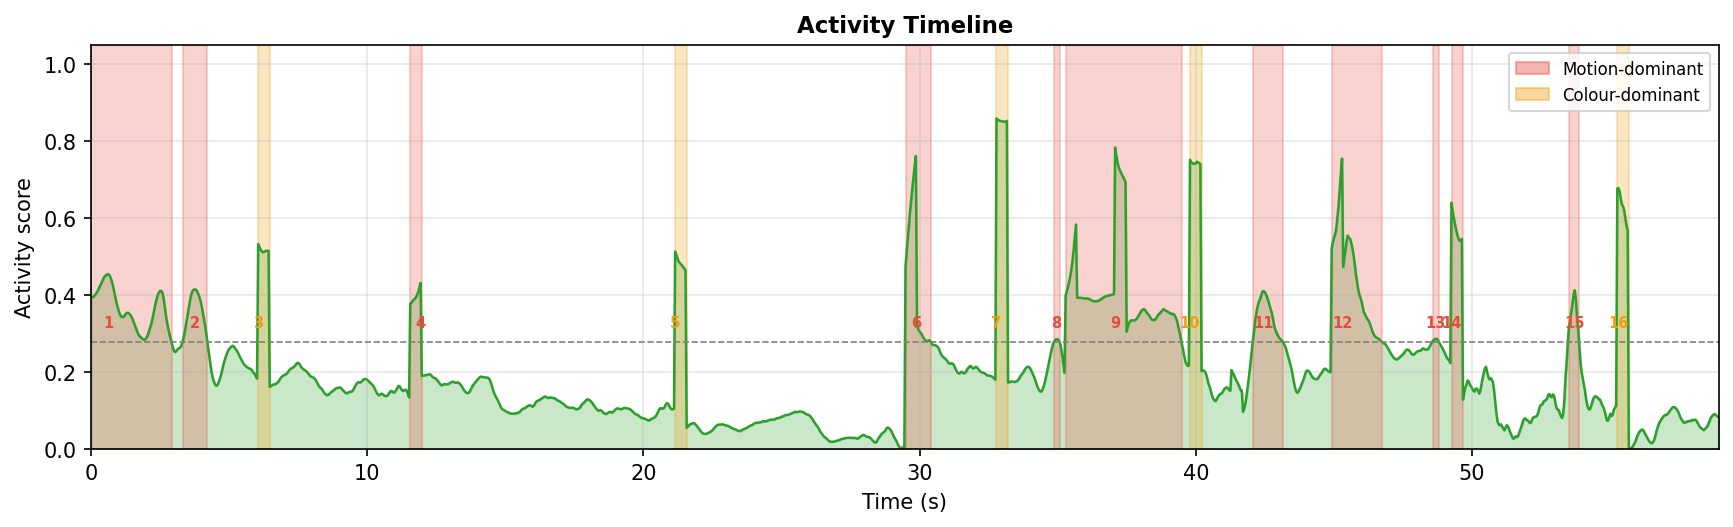
\includegraphics[width=\textwidth]{plots/data_octopus/activity_timeline.png}
    \caption{Combined activity score over the full clip with numbered event
             labels. Red spans are motion-dominant; orange spans are
             colour-dominant.}
\end{figure}

% ─────────────────────────────────────────────────────────────────────────────
\section{Analysis}

The two features provide complementary windows into cephalopod behavioral
state. Motion magnitude quantifies locomotor activity, capturing transitions
between resting, slow crawling, and rapid escape or hunting behavior.
Histogram change is particularly relevant for cephalopods because it tracks
dynamic skin patterning produced by chromatophores, iridophores, and
papillae — structures known to encode emotional and communicative signals.
In this clip, early spikes in histogram change coincide with elevated motion,
consistent with the animal actively repositioning in response to stimuli.
Subsequent motion fluctuations with more stable histograms suggest
lower-intensity locomotion without strong camouflage adjustments.

The main limitations are sensitivity to camera movement and uncontrolled
backgrounds, both of which produce false positives unrelated to animal
behaviour. Averaging pixel values over the full frame also conflates animal
activity with environmental noise — foreground segmentation would
substantially improve signal quality. At $\sim$24\,fps, rapid chromatophore
flickers may also be temporally aliased, and slow tonal gradients require
longer recordings to detect reliably.

Integrating additional modalities would greatly enrich the analysis. 3D pose
estimation via deep learning keypoint models would add fine-grained body
posture features linked to specific behavioral states such as threat displays
or mating dances. Hydrophone or audio signals could detect jet propulsion
bursts correlated with escape responses. Combining these signals with temporal
context models — for example Hidden Markov Models or LSTMs — would enable
reliable, automatic behavioural state segmentation with far greater specificity.

% ─────────────────────────────────────────────────────────────────────────────
\section{Reproducibility}

All code is available in the accompanying repository. To reproduce:

\begin{enumerate}
    \item Create and activate the virtual environment: \texttt{source env/bin/activate}
    \item Install dependencies: \texttt{pip install -r requirements.txt}
    \item Download and prepare the video (see \texttt{README.md})
    \item Run \texttt{python analyze.py} to extract features and generate plots
    \item Open \texttt{cephalopod\_analysis.ipynb} for the full annotated pipeline
    \item Open \texttt{activity\_visualization.ipynb} for activity event exploration
\end{enumerate}

\end{document}
